\documentclass[11pt]{article}
\usepackage[margin=1in]{geometry}
\usepackage{amsmath,amssymb}
\usepackage{lmodern}
\usepackage[T1]{fontenc}
\usepackage{enumitem}
\usepackage{microtype}
\usepackage{tikz}
\usetikzlibrary{arrows.meta,angles,quotes,calc,decorations.pathreplacing,patterns}

\title{2011 F=ma Exam Review}
\author{Nathan P.}
\date{December 23, 2025}

\begin{document}
\maketitle

\section*{Problem 6}
The $v'=\dfrac{2mv}{M+m}$ formulas are only for elastic collisions. This was a perfectly inelastic collision, so $mv_c=4mv$ and $v=v_c/4$.

\section*{Problem 12}
Key idea: rods only exert force along their axis.
Superposition: the forces between A and B, or A and C, can be added, but they can also be treated independently of each other.
The compressive force in each rod is still $F$. It cannot be less, otherwise the masses would not have enough force to be held apart. There's a mass vertically in between two of the masses, so you might intuitively think the force the rod has to exert is greater than $F$. However, when you consider the symmetry, the compression in the rods cannot be greater than $F$, because if they were all greater than $F$, the masses would be pushed apart, since the force between any two is only $F$.

\section*{Problem 13}
This question is asking at what $\theta$ it will stop rolling to the right. Basically, what's the static equilibrium condition? If $\theta$ is too large, it rolls to the right. If $\theta$ is too small, it would slip.
Balancing torques and forces gives
\[
Tr=fR,\qquad T\cos\theta=f,
\]
leading to $\cos\theta=r/R=1/2$, and our answer of $\theta=60^\circ$.

\begin{center}
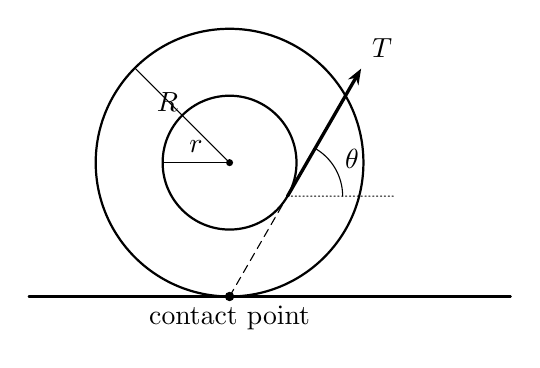
\begin{tikzpicture}[scale=0.85, line cap=round, line join=round, >={Stealth[length=2mm]}]
  % R = 2, r = 1, theta = 60: the thread's line passes through the contact point
  \draw[thick] (-3,0) -- (4.2,0);
  \draw[thick] (0,2) circle (2);
  \draw[thick] (0,2) circle (1);
  \fill (0,2) circle (1.5pt);
  \coordinate (Q) at ({sin(60)},{2-cos(60)});
  \draw[->, very thick] (Q) -- ++(60:2.2) node[above right] {$T$};
  \draw[densely dashed] (0,0) -- (Q);
  \fill (0,0) circle (2pt) node[below] {contact point};
  \coordinate (Qh) at ($(Q)+(1.6,0)$);
  \coordinate (Qt) at ($(Q)+(60:1)$);
  \draw[densely dotted] (Q) -- (Qh);
  \pic[draw, "$\theta$", angle radius=7mm, angle eccentricity=1.35] {angle = Qh--Q--Qt};
  \draw (0,2) -- (-1,2) node[midway, above] {$r$};
  \draw (0,2) -- (-1.414,3.414) node[midway, above left=-2pt] {$R$};
\end{tikzpicture}
\end{center}

\section*{Problem 14}
Picture it carefully: the weights hit the ground from bottom to top, and the weights should be more spaced out the higher you go.
Spaced out by how much? $d\propto t^2$, so if you travel $d$ in the first second, you travel $3d$ in the 2nd second, $5d$ in the third second, and in the 4th second $16d-9d=7d$. The intervals should be $1,3,5,7,\ldots$

\begin{center}
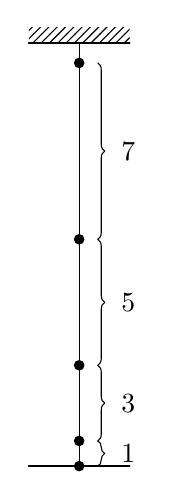
\begin{tikzpicture}[scale=0.32, line cap=round, line join=round]
  \draw[thick] (-2,16.8) -- (2,16.8);
  \fill[pattern=north east lines] (-2,16.8) rectangle (2,17.4);
  \draw[thick] (-2,0) -- (2,0);
  \draw (0,16.8) -- (0,0);
  \foreach \y in {0,1,4,9,16} \fill (0,\y) circle (6pt);
  \foreach \a/\b/\l in {0/1/1,1/4/3,4/9/5,9/16/7}
    \draw[decorate, decoration={brace, mirror, raise=4pt}] (0.3,\a) -- (0.3,\b) node[midway, right=9pt] {$\l$};
\end{tikzpicture}
\end{center}

\section*{Problem 18}
Energy conservation is the right method here, so if the answer comes out wrong, it's the algebra. Draw out the problem and clearly write the steps.
If you see that your answer isn't even among the options, try looking through your work to spot errors, not trying to verify your incorrect answer, because it's incorrect! If it'd be fast, skip the problem and redo it later so you forget your incorrect method.

\section*{Problem 19}
Given the vector components of $F$, you may treat $F$ in the $x$ and $y$ directions as separate.
It's in the form $F=-k(x\,\hat\imath+y\,\hat\jmath)$, meaning the particle undergoes SHM in the $x$ and $y$ directions. It's like a diagonal spring.
You're also given the $v$ vector components at the origin (where $v$ is at a max).
We're asked for the time for the particle to return to the origin, which happens at $T/2$, because that's how SHM works (think of the sinusoidal graph).

\section*{Problem 20}
We're asked for the max distance, or amplitude, which we can relate to the max velocity by energy conservation.
Luckily, we're given $v_{\max}$, which happens at the origin.
Solve for $A$ by treating energy independently in the $x$ and $y$ directions, and use Pythagoras to get $A$ from $x_{\max}$ and $y_{\max}$.

\section*{Problem 24}
A teflon ring is just a ring.
The question asks about the power to overcome friction and rotate at a constant rate, meaning the force is just enough to balance friction.
It says that $\omega$, the weight of the turntable, and $\mu$ stay constant.
\[
P=Fv=\mu N\cdot R\omega=\mu W\cdot R\omega
\]
($N$ balances $W$, and friction is the same because the weight doesn't change).
Increasing $\delta$ only increases the width of the bearing, which doesn't do much because it's way thinner than $R$.
Increasing $R$, on the other hand, increases the power ($P\propto R$), because it takes more power to get $v$ higher (greater $R$ means greater $v$ on the rim).

\section*{Problem 25}
When time's involved, you must use something like the UAM equations or impulse.

\end{document}
